% Permission is granted to copy, distribute and/or modify this document
% under the terms of the GNU Free Documentation License, Version 1.3
% or any later version published by the Free Software Foundation;
% with no Invariant Sections, no Front-Cover Texts, and no Back-Cover Texts.
% A copy of the license is included in the section entitled "GNU
% Free Documentation License".
%
% Written (C) 2012-2013 Heiko Strathmann

\section{Independence Testing with the HSIC Statistic}
\label{sec:hsic_test}

Independence testing tries to solve the following problem (taken from \citep{Gretton2008d}):
Let $\textbf{P}_{xy}$ be a Borel probability measure defined on a domain $\mathcal{X}\times\mathcal{Y}$, and let $\textbf{P}_x$ and $\textbf{P}_y$ be the respective marginal distributions on $\mathcal{X}$ and $\mathcal{Y}$. Given samples $Z=(X,Y)=\{(x_1, y_1), ..., (x_m, y_m)\}$ of size $m$ drawn independently and identically distributed according to $\textbf{P}_{xy}$, does $\textbf{P}_{xy}$ factorise as $\textbf{P}_{xy}=\textbf{P}_x \textbf{P}_y$? This corresponds to the question: Are $\textbf{P}_x$ and $\textbf{P}_y$ statistically independent? An independence test will distinguish between the hypothesises
\begin{align*}
H_0: \textbf{P}_{xy}=\textbf{P}_x \textbf{P}_y\\
H_1: \textbf{P}_{xy}\neq\textbf{P}_x \textbf{P}_y\\
\end{align*}

As for two-sample-testing, it is desirable to have a statistic that is zero if and only if $\textbf{P}_x$ and $\textbf{P}_y$ are independent. The so-called \emph{Hilbert Schmidt Independence Criterion} has this property. It is the squared Hilbert-Schmidt norm of the cross-covariance operator. We will now briefly describe where it comes from.

Let $\mathcal{F}$ be a RKHS with continuous feature mapping $\phi:\mathcal{X}\rightarrow\mathcal{F}$ and kernel $k:\mathcal{X}\times\mathcal{X}\rightarrow\mathbb{R}$ such that $\langle \phi(x)\phi(x')\rangle_\mathcal{F}=k(x,x')$; let $\mathcal{G}$ be another RKHS with continuous feature mapping $\psi:\mathcal{X}\rightarrow\mathcal{G}$ and kernel $l:\mathcal{Y}\times\mathcal{Y}\rightarrow\mathbb{R}$ such that $\langle \psi(y)\psi(y')\rangle_\mathcal{G}=k(y,y')$. The cross-covariance operator $C_{xy}:\mathcal{G}\rightarrow\mathcal{F}$ is defined such that for all $f\in\mathcal{F}$ and $g\in\mathcal{G}$
\begin{align*}
\langle f,C_{xy}g \rangle_\mathcal{F}=\textbf{E}_{xy}([f(x)-\textbf{E}_x(f(x))][g(y)-\textbf{E}_y (g(y))]
\end{align*}
The operator itself can be written as
\begin{align*}
C_{xy}=\textbf{E}_{xy}(\phi(x)-\mu_x) \otimes
 (\psi(y) - \mu_y)]
\end{align*}
where $\otimes$ is the tensor product. This is the generalisation of the cross-covariance matrix between random vectors in a RKHS. When $\mathcal{F}$ and $\mathcal{G}$ are \emph{universal}, then $||C_{xy}||$ is z is zero if and only if $H_0:\textbf{P}_{xy}=\textbf{P}_x \textbf{P}_y$ holds. Collecting everything gives the population expression for the HSIC. Let $x', y'$ be independent copies of the random variables $x,y$ respectively.
\begin{align}
\label{eqn:hsic_population}
\hsic[\textbf{P}_{xy},\mathcal{F},\mathcal{G}]=\textbf{E}_{xx'yy'}[k(x,x')l(y,y')] &+ \textbf{E}_{xx'}[k(x,x')]\textbf{E}_{yy'}[l(y,y')]\\
&-2\textbf{E}_{xy}[\textbf{E}_{x'}[k(x,x')]\textbf{E}_{y'}[l(y,y')]\notag
\end{align}

See \citep{Gretton2008d} for details. \shogun{} implements a biased estimator of the HSIC along with various methods to approximate its null distribution.

\subsection{Estimate of HSIC}
We now describe the method to estimate the HSIC that is implemented in \shogun{}, as described in \citep[Equation 4]{Gretton2008d}. All methods are implemented in \shogunclass{CHSIC}. The HSIC statistic has quadratic time and space costs, since it involves computing full kernel matrices and centring them.

A biased estimator for expression \ref{eqn:hsic_population} is given by
\begin{align*}
\hsic_b[(X,Y),\mathcal{F},\mathcal{G}]=\frac{1}{m^2}\trace(\textbf{KHLH})
\end{align*}
where $\textbf{K}, \textbf{L}$ are the full kernel matrices of kernels $k, l$ respectively and $\textbf{H}=\textbf{I}-\frac{1}{m}\textbf{1}\textbf{1}^T$ is a centring matrix with $\textbf{1}$ being a $m\times m$ matrix of ones. In \shogun{}, this expression is not evaluated using matrix multiplication, but the centring is done by hand. Call \texttt{compute\_statistic} in order to compute the estimate. Note that the method returns $m\hsic_b[(X,Y),\mathcal{F},\mathcal{G}]$ since null distribution approximations work on $m$ times null distribution.

\subsubsection{Bootstrapping}
As for any independence test in \shogun{}, bootstrapping can be used to approximate the null-distribution with any type of statistic. This results in a consistent, but slow test. Note that for each sample, the HSIC estimate has to be re-computed. The number of samples to take is the only parameter. As a rule of thumb, use at least 250 samples.
See \texttt{bootstrap\_null} in \shogunclass{CTwoDistributionsTestStatistic}, \shogunclass{CKernelIndependenceTestStatistic}, and \shogunclass{CHSIC}. Note that since the full kernel matrices have to be stored anyway when computing the HSIC estimate, in \texttt{bootstrap\_null}, these are pre-computed automatically for the current bootstrapping instance.
Bootstrapping is the only consistent HSIC test that is implemented in \shogun{}.

\subsubsection{Gamma}
Another, fast but heuristic method for approximating the null distribution for the HSIC is by matching the first two moments of a gamma distribution to it \citep[Equation 9]{Gretton2008d}. This is not consistent but usually gives good results in practice. However, there are distributions which break the gamma test. Therefore, the type I error should always be monitored.

It uses
\begin{align}
\label{eqn:hsic_gamma}
m\hsic_b(Z) \sim \frac{x^{\alpha-1}\exp(-\frac{x}{\beta})}{\beta^\alpha \Gamma(\alpha)}
\end{align}
where
\begin{align*}
\alpha=\frac{(\textbf{E}(\hsic_b(Z)))^2}{\var(\hsic_b(Z))} \qquad \text{and} \qquad
 \beta=\frac{m \var(\hsic_b(Z))}{(\textbf{E}(\hsic_b(Z)))^2}
\end{align*}

Then, any threshold and p-value can be computed using the gamma distribution in expression \ref{eqn:hsic_gamma}. Computational costs are in $\mathcal{O}(m^2)$, similar for space.

To use that method for testing, use \texttt{set\_null\_approximation\_method(HSIC\_GAMMA)}, to be found in \shogunclass{CHSIC}.

\subsubsection{Kernel Selection}
Kernel selection for HSIC-based tests is an ongoing subject of research. In the near future, recent results on this topic will be implemented into \shogun{}. In the meantime, a good heuristic to start with, when using a Gaussian kernel as implemented in \shogunclass{CGaussianKernel}, is to use the median distance in the underlying data as kernel bandwidth. This way, the kernel captures at least the scaling of underlying data. In many cases, this leads to usable first results, however, the method may badly fail if signal is hidden at another length scale than the one of the overall data. The method is mentioned in \citep[Appendix C]{Gretton2012}.

In order to do this, note that  \shogun{}'s Gaussian kernel implementation uses a different parametrization as most other literature:
\begin{align*}
k(x,x')=\exp\left( \frac{||x-x'||_2^2}{\tau}\right)
\end{align*}
where $\tau$ is the width that is passed to the constructor of \shogunclass{CGaussianKernel}. In order to translate a median distance $d$ to this kernel, simply pass $\tau=d^2$.

\shogun{} implements classes that can compute median distances. Create an instance of the class \shogunclass{CEulideanDistance}, call the method \texttt{distance\_matrix} to compute all pairwise distances of passed data. Then, use the method \texttt{matrix\_median} of  \shogunclass{CStatistics} in order to compute the median of all elements in the matrix. Store this distance and pass it to the Gaussian kernel as described above.

Note that the median is a very stable statistic, therefore, it is not necessary to compute all pairwise distances. A subset of a few hundred points is sufficient. This can be done via setting a subset to the instance of \shogunclass{CFeatures} that holds the data. To do so, create a random index permutation via calling method \texttt{randperm\_vec} of class \shogunclass{CMath}, and only keep the $n$ first indices where $n$ is the number of distances that should be computed. Call \texttt{add\_subset} on the instance of \shogunclass{CFeatures} that holds the data and give the indices as parameter. Then, this instance can be passed to \shogunclass{CEulideanDistance} as described above. Distances will only be computed for specified indices. Once the distance matrix is computed, call \texttt{remove\_subset} to reset the original state of the data.

The whole procedure is included in all python examples, including the graphical ones. Note that since there is a kernel for each distribution, two kernel parameters have to be selected. Using the described median heuristic also leads to good results in some cases, as mentioned in \citep{Gretton2008d}.

\subsubsection{Example}
There is a graphical python example which plots example data, alternative and null-distributions. See figure \ref{fig:statistical_testing-hsic}.

\begin{figure}\centering
		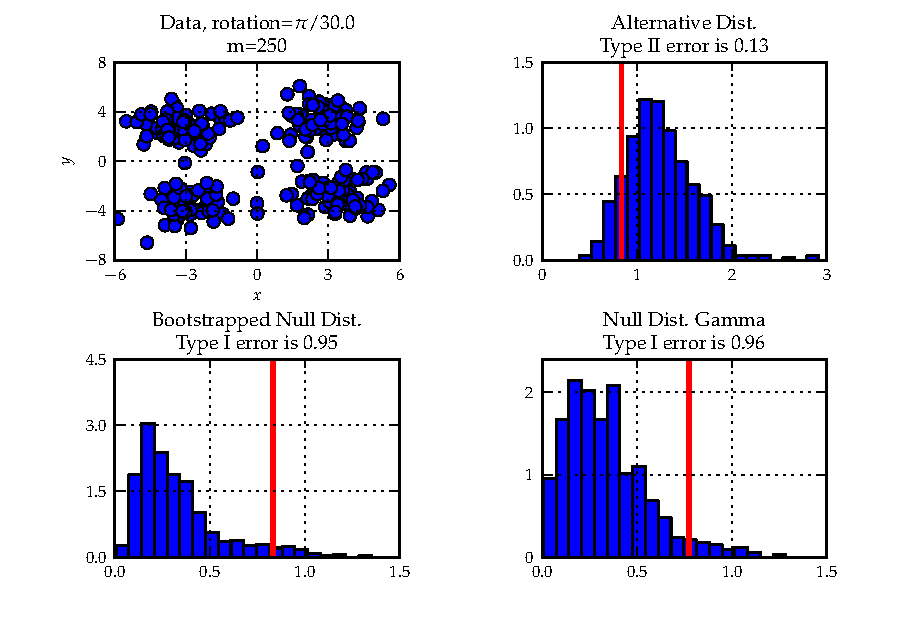
\includegraphics{fig/statistical_testing/hsic}
		\caption{Screenshot of graphical python example for HSIC.}
		\label{fig:statistical_testing-hsic}
\end{figure}